\documentclass[aspectratio=169,10pt]{beamer}

% ========== Packages ==========
\usepackage[utf8]{inputenc}
\usepackage{amsmath, amssymb}
\usepackage{xcolor}
\usepackage{tikz}
\usetikzlibrary{arrows.meta}
\usepackage{graphicx}
\usepackage{booktabs}

% ========== Theme ==========
\usetheme{metropolis}

% ========== Dark navy color ==========
\definecolor{navymain}{RGB}{26, 43, 76}        % deep navy
\definecolor{navylight}{RGB}{200, 210, 225}    % light tint for backgrounds
\definecolor{accentred}{RGB}{180, 60, 60}      % muted red for warnings
\definecolor{winner}{RGB}{30, 110, 60}         % muted green for best cells

\setbeamercolor{frametitle}{bg=navymain, fg=white}
\setbeamercolor{title separator}{fg=navymain}
\setbeamercolor{progress bar}{fg=navymain}
\setbeamercolor{alerted text}{fg=accentred}
\setbeamercolor{block title}{bg=navymain, fg=white}
\setbeamercolor{block body}{bg=navylight!30, fg=black}
\setbeamercolor{normal text}{fg=black}
\setbeamercolor{itemize item}{fg=navymain}
\setbeamercolor{itemize subitem}{fg=navymain}
\setbeamercolor{section in toc}{fg=navymain}

% ========== Title info ==========
\title{Lab Meeting}
\date{2026.07.16}
\author{Sunghyun Choi}

\begin{document}

% ========== Slide 1: Title ==========
\begin{frame}[plain]
    \vspace{1.2cm}
    \begin{center}
        {\fontsize{26}{32}\selectfont\bfseries\color{navymain} Lab Meeting}

        \vspace{0.4cm}
        {\fontsize{18}{22}\selectfont 2026.07.16}

        \vspace{0.4cm}
        {\fontsize{14}{18}\selectfont\itshape\color{black!70} Sunghyun Choi}
    \end{center}
\end{frame}

% ========== Slide 2: Recap 1 -- the question ==========
\begin{frame}{Recap --- Where Does MAD Fit?}
    \vspace{0.5cm}
    Multi-Agent Debate is studied mostly in \textbf{reasoning} --- math,
    factuality, QA. But at its core it is one thing: an
    \textbf{interaction of differing perspectives}.

    \vspace{0.5cm}
    Fuzzy objectives (\emph{good design}, \emph{compelling writing}) have
    \textbf{no ground truth}, and are usually optimized by compressing many
    preferences into \textbf{one scalar} --- a reward model, or a single
    LLM-as-judge.

    \vspace{0.6cm}
    \begin{block}{The Question (last meeting)}
        Can a well-designed \textbf{MAD harness} --- many perspectives in
        debate --- optimize these fuzzy objectives better?
    \end{block}
\end{frame}

% ========== Slide 3: Recap 2 -- the harness ==========
\begin{frame}{Recap --- Starting Point: Anthropic's Harness}
    \vspace{0.5cm}
    The blog optimizes something that \emph{cannot be quantified} --- frontend
    \textbf{design quality} --- with a \textbf{generator--evaluator loop}: one
    agent builds the page, another grades and critiques it, and the critique
    drives the next version.

    \vspace{0.4cm}
    The trick is making ``beautiful'' gradable:
    \textbf{functionality} $\cdot$ \textbf{design} $\cdot$
    \textbf{originality} $\cdot$ \textbf{craft}.

    \vspace{0.5cm}
    \begin{alertblock}{The gap $\to$ this work}
        The blog collapses all four into \textbf{one fused evaluator}.
        We un-collapse it: \textbf{one expert critic per criterion}, let them
        \textbf{debate}, and a moderator synthesizes their verdicts.
    \end{alertblock}
\end{frame}

% ========== Slide 4: Experiment design -- arms ==========
\begin{frame}{Experiment Design --- Arms as a Ladder}
    \vspace{0.3cm}
    Each arm adds \textbf{one ingredient} over the one above it.

    \vspace{0.5cm}
    \centering
    \small
    \begin{tabular}{@{}ll@{}}
        \toprule
        \textbf{Arm} & \\
        \midrule
        ZS    & (zero-shot, one pass) \\
        SELF  & (self-critique loop) \\
        FUSED & (one external fused evaluator) \\
        AXES  & (per-axis critics, no debate) \\
        \textbf{MAD}   & (per-axis critics $+$ debate) \\
        \bottomrule
    \end{tabular}

    \vspace{0.5cm}
    \raggedright
    {\footnotesize \textbf{Consensus-stop}: each loop stops when its own evaluator
    says \emph{good enough}. (Max round = 10)}
\end{frame}

% ========== WebGen measurement (from previous deck) ==========
\begin{frame}{Dataset --- WebGen-Bench}
    \vspace{0.2cm}
    \begin{columns}[T]
    \column{0.42\textwidth}
    \vspace{0.4cm}
    Two independent axes per website:
    \begin{itemize}
        \setlength{\itemsep}{0.3cm}
        \item \textbf{Functionality} \\
              {\footnotesize a UI agent operates the site --- objective,
              execution-grounded}
        \item \textbf{Appearance} \\
              {\footnotesize an LLM judge grades design on a \textbf{1--5} scale}
    \end{itemize}

    \vspace{0.4cm}

    \column{0.58\textwidth}
    \centering
    \vspace{0.1cm}
    \includegraphics[width=\linewidth]{img/appearance_crop.png}

    \vspace{0.1cm}
    {\scriptsize Appearance score examples (1--5).}
    \end{columns}
\end{frame}

% ========== WebGen result: models (left) + final table (right) ==========
\begin{frame}{Results}
    \vspace{0.9cm}
    \begin{center}
    \begin{minipage}[t]{0.34\textwidth}
        \vspace{0pt}
        \textbf{Setup}
        \small
        \begin{itemize}
            \setlength{\itemsep}{0.1cm}
            \item generator $=$ critic: \\ \textbf{Qwen2.5-VL-32B}
            \item held-out judge: \\ \textbf{Qwen2.5-VL-72B}
        \end{itemize}
    \end{minipage}%
    \hspace{1.4cm}%
    \begin{minipage}[t]{0.26\textwidth}
        \vspace{0pt}
        \centering
        \begin{tabular}{@{}lc@{}}
            \toprule
            \textbf{Arm} & \textbf{score} \\
            \midrule
            ZS    & 5.11 \\
            SELF  & 4.95 \\
            FUSED & 5.46 \\
            \textbf{AXES}  & \color{winner}\textbf{5.68} \\
            MAD   & 5.58 \\
            \bottomrule
        \end{tabular}
    \end{minipage}
    \end{center}
\end{frame}

% ========== Analysis 1: design churn -- FUSED preserves, MAD rewrites ==========
\begin{frame}{FUSED Preserves the Design --- MAD Rewrites It}
    \vspace{0.5cm}
    \centering
    {\footnotesize\textbf{FUSED}}\\[3pt]
    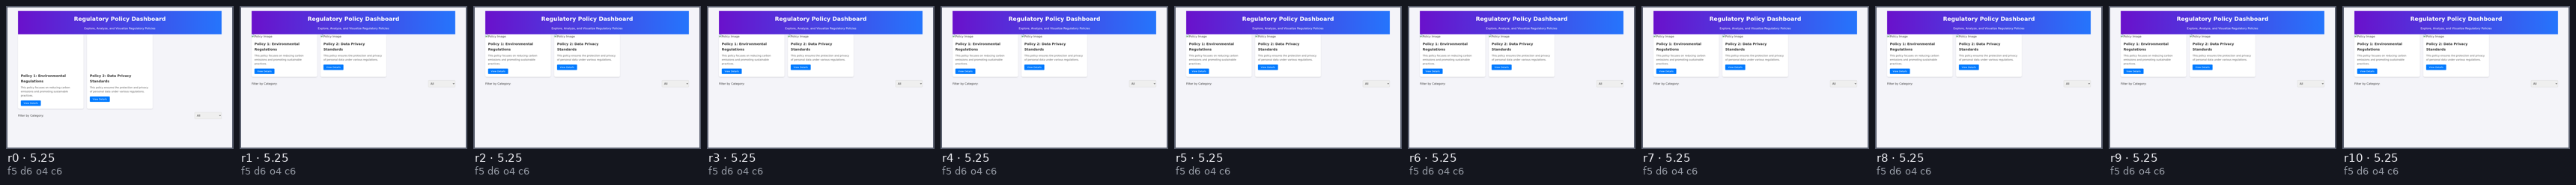
\includegraphics[width=0.92\linewidth]{img/churn_000005_FUSED.png}

    \vspace{0.7cm}
    {\footnotesize\textbf{MAD}}\\[3pt]
    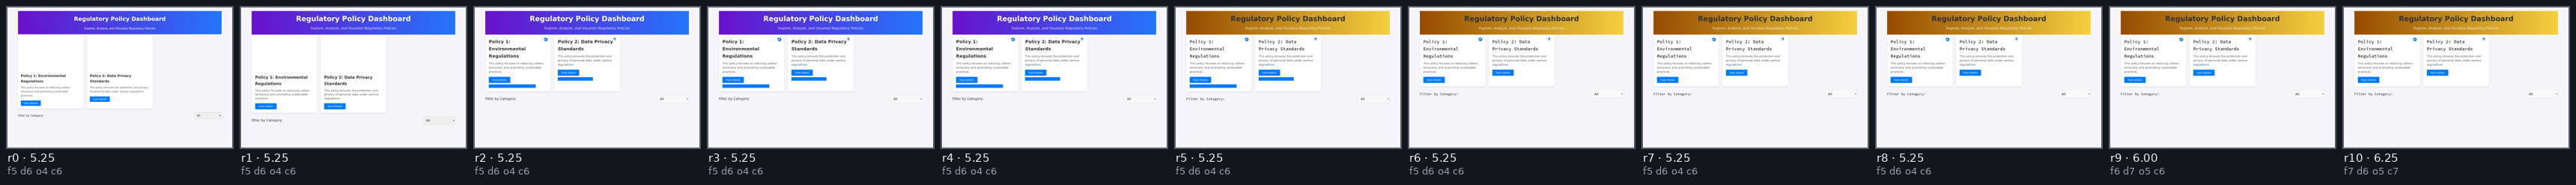
\includegraphics[width=0.92\linewidth]{img/churn_000005_MAD.png}
\end{frame}

% ========== Analysis 2: MAD peaks early but never stops ==========
\begin{frame}{MAD Peaks Early --- but Never Stops}
    \vspace{0.3cm}
    \centering
    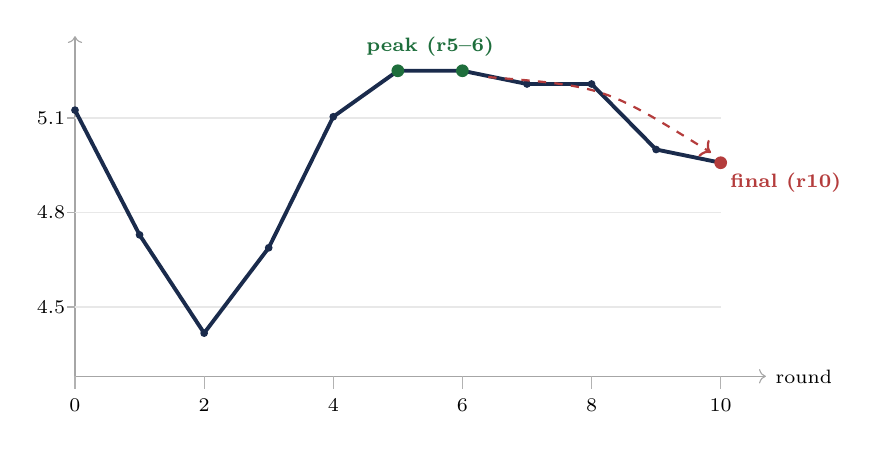
\begin{tikzpicture}[x=0.82cm,y=4.0cm]
        % axes
        \draw[->,gray!70] (0,-0.02) -- (10.7,-0.02) node[right,black,font=\scriptsize]{round};
        \draw[->,gray!70] (0,-0.02) -- (0,1.06);
        \foreach \yy/\lab in {0.2/4.5, 0.5/4.8, 0.8/5.1}{
            \draw[gray!60] (-0.12,\yy)--(0,\yy) node[left,black,font=\scriptsize]{\lab};
            \draw[gray!18] (0,\yy)--(10,\yy);
        }
        \foreach \xx in {0,2,4,6,8,10}
            \draw[gray!60] (\xx,-0.02)--(\xx,-0.06) node[below,black,font=\scriptsize]{\xx};
        % MAD mean-overall curve (ArtifactsBench, Qwen3-VL-32B, n=12)
        \draw[navymain,line width=1.4pt]
            (0,0.825)--(1,0.429)--(2,0.117)--(3,0.388)--(4,0.804)--(5,0.95)--(6,0.95)--(7,0.908)--(8,0.908)--(9,0.7)--(10,0.658);
        \foreach \p in {(0,0.825),(1,0.429),(2,0.117),(3,0.388),(4,0.804),(7,0.908),(8,0.908),(9,0.7)}
            \fill[navymain] \p circle (1.4pt);
        % peak (early-mid)
        \fill[winner] (5,0.95) circle (2.3pt);
        \fill[winner] (6,0.95) circle (2.3pt);
        \node[winner,font=\scriptsize\bfseries,above] at (5.5,0.965){peak (r5--6)};
        % degrade to the cap
        \draw[->,accentred,thick,dashed] (6.4,0.93) .. controls (8.2,0.9) .. (9.85,0.69);
        \fill[accentred] (10,0.658) circle (2.3pt);
        \node[accentred,font=\scriptsize\bfseries,below right] at (10,0.658){final (r10)};
    \end{tikzpicture}

    \vspace{0.25cm}
    \raggedright
    
\end{frame}

% ========== ArtifactsBench dataset ==========
\begin{frame}{Dataset --- ArtifactsBench}
    \vspace{0.2cm}
    \begin{columns}[T]
    \column{0.54\textwidth}
    \vspace{0.2cm}
    A benchmark of \textbf{prompts asking an LLM to build a web artifact}
    --- a game, an SVG scene, an interactive dashboard, a simulation.

    \vspace{0.5cm}
    \begin{block}{Why it fits us}
        \footnotesize
        \begin{itemize}
            \setlength{\itemsep}{0.2cm}
            \item design-forward tasks $\to$ lots of \emph{subjective} room,
                  where debate should matter
            \item one HTML file, offline $\to$ easy to render, probe, and
                  judge at scale
        \end{itemize}
    \end{block}

    \column{0.46\textwidth}
    \centering
    \vspace{0.1cm}
    \begin{block}{Example prompt}
        \footnotesize\itshape ``Write a frontend program that simulates the
        moon's rotation.''
    \end{block}

    \vspace{0.1cm}
    \begin{tikzpicture}
        \node[draw=navymain, line width=1pt, inner sep=0pt]{%
            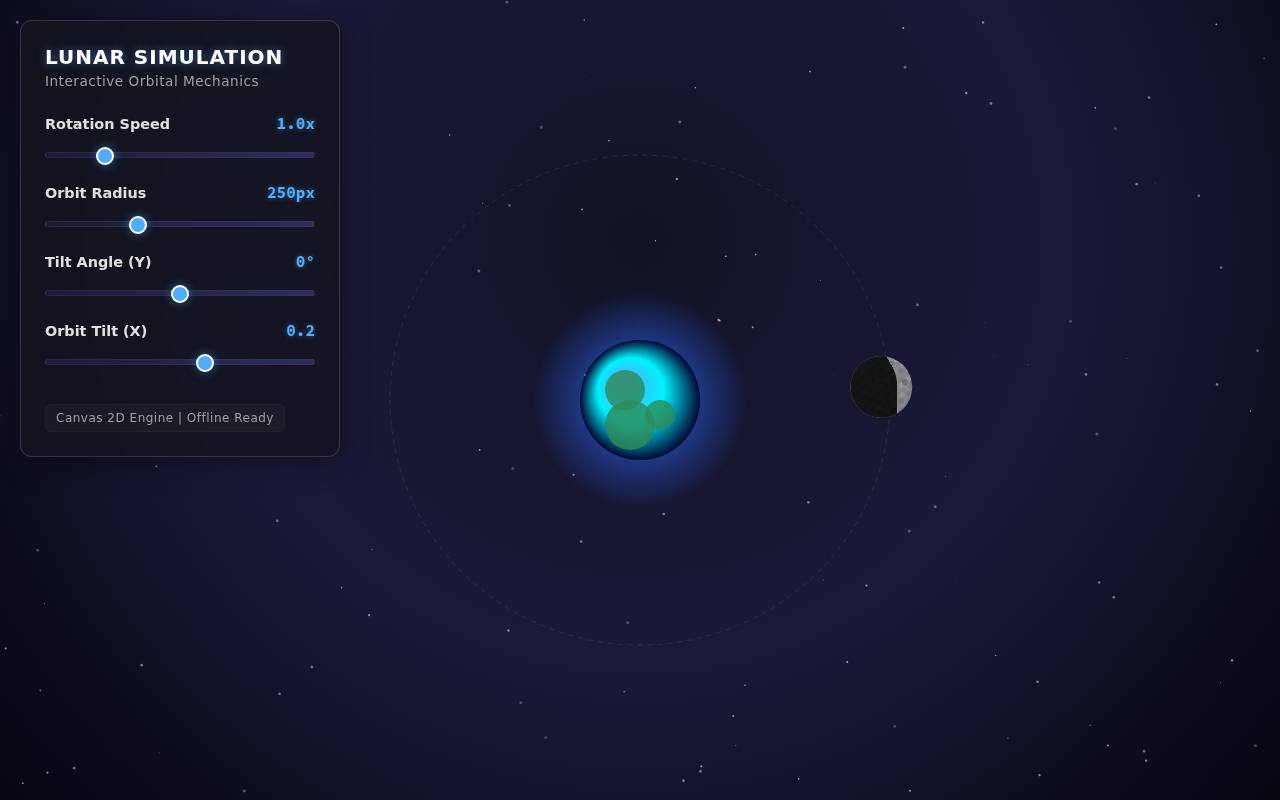
\includegraphics[width=\linewidth]{img/moon_r4_good.png}};
    \end{tikzpicture}

    \vspace{0.1cm}
    {\scriptsize rendered result --- a working Canvas 2D simulation}
    \end{columns}
\end{frame}

% ========== ArtifactsBench result: single VLM-only setup ==========
\begin{frame}{Results}
    \vspace{0.9cm}
    \begin{center}
    \begin{minipage}[t]{0.34\textwidth}
        \vspace{0pt}
        \textbf{Setup}
        \small
        \begin{itemize}
            \setlength{\itemsep}{0.1cm}
            \item generator $=$ critic: \\ \textbf{Qwen3-VL-32B}
            \item held-out judge: \\ \textbf{Qwen3-VL-32B}
        \end{itemize}

        \vspace{0.15cm}
    \end{minipage}%
    \hspace{1.4cm}%
    \begin{minipage}[t]{0.26\textwidth}
        \vspace{0pt}
        \centering
        \begin{tabular}{@{}lc@{}}
            \toprule
            \textbf{Arm} & \textbf{score} \\
            \midrule
            ZS    & 5.12 \\
            SELF  & 5.12 \\
            \textbf{FUSED} & \color{winner}\textbf{5.29} \\
            AXES  & 4.79 \\
            MAD   & 4.92 \\
            \bottomrule
        \end{tabular}
    \end{minipage}
    \end{center}
\end{frame}

% ========== Ongoing: grounding the debate axes in HCI theory ==========
\begin{frame}{Ongoing --- Which Axes Should the Critics Debate?}
    \vspace{0.3cm}
    \begin{columns}[T]
    \column{0.60\textwidth}
    \small
    \begin{itemize}
        \setlength{\itemsep}{0.32cm}
        \item \textbf{VisAWI} \ {\footnotesize (Moshagen \& Thielsch 2010)} ---
              validated structure of website aesthetics: \emph{simplicity
              $\cdot$ diversity $\cdot$ colorfulness $\cdot$ craftsmanship}.
        \item \textbf{Classical / Expressive} \ {\footnotesize (Lavie \&
              Tractinsky 2004)} --- two-factor: \emph{order \& clarity} vs.
              \emph{creative, expressive}.
        \item \textbf{Pragmatic / Hedonic} \ {\footnotesize (Hassenzahl,
              AttrakDiff)} --- \emph{does it work} vs. \emph{stimulation}
              \& \emph{identity}.
    \end{itemize}

    \vspace{0.25cm}
    {\footnotesize Swap \emph{only} the critic axes; generator, judge and
    stop rule held fixed.}

    \column{0.36\textwidth}
    \vspace{0.5cm}
    \centering
    {\footnotesize MAD --- final overall}

    \vspace{0.15cm}
    \small
    \begin{tabular}{@{}lc@{}}
        \toprule
        \textbf{axis set} & \textbf{overall} \\
        \midrule
        blog 4 axes         & 6.58 \\
        VisAWI              & 6.62 \\
        Lavie--Tractinsky   & 6.92 \\
        \textbf{Hassenzahl} & \color{winner}\textbf{6.93} \\
        \bottomrule
    \end{tabular}

    \vspace{0.25cm}
    {\scriptsize ArtifactsBench, $n{=}15$ \\ held-out VL-72B \\ \emph{early --- not yet significant}}
    \end{columns}
\end{frame}

% ========== References ==========
\begin{frame}{References}
    \vspace{0.4cm}
    \footnotesize
    \begin{enumerate}
        \setlength{\itemsep}{0.3cm}
        \item Du, Y., et al. (2023). \textit{Improving Factuality and Reasoning
              through Multiagent Debate.} arXiv:2305.14325.
        \item Zhang, H., et al. (2025). \textit{Stop Overvaluing Multi-Agent
              Debate.} arXiv:2502.08788.
        \item Tencent Hunyuan (2025). \textit{ArtifactsBench.} arXiv:2507.04952.
        \item Lu, Z., et al. (2025). \textit{WebGen-Bench.} arXiv:2505.03733.
        \item Rajasekaran, P. (2026). \textit{Harness Design for Long-Running
              Application Development.} Anthropic Engineering Blog.
        \item Moshagen \& Thielsch (2010), \textit{VisAWI}, IJHCS; \quad
              Lavie \& Tractinsky (2004), \textit{Web aesthetics dimensions},
              IJHCS.
    \end{enumerate}
\end{frame}

\end{document}
